\section{Protection vers le microscope}
Cette section va expliquer les différentes étapes de la conception de la protection vers le microscope, la
modélisation de celle-ci, les prototypes qui ont été réalisés, la fabrication final ainsi
que le montage.
\subsection{Réflexion préliminaire}
Contrairement à la précédente protection, la table croisée bouge dans l'espace sur les trois axes X,Y et Z. Il faut, dans ce cas, trouvé un moyen de faire une protection qui puisse être mobile afin de supporter les efforts dans toutes les directions. La table peut se déplacer d'environ 12~mm en X et Y, et de 25~mm en Z.

La première approche s'est tournée vers de l'impression 3D de plastique souple, tel que du TPU. Ses propriétés élastiques permettent d'avoir une certaine liberté de mouvement.

Les Figures~\ref{zigzag_model}~et~\ref{zigzag_reel}, ci-contre, illustrent un modèle 3D de test avec une géométrie en \textit{zigzag}, afin de tester ses propriétés élastiques. Ce modèle n'a pas du tout été concluant, la structure est beaucoup trop rigide en élasticité.

\begin{minipage}[c]{0.48\textwidth}
    \begin{center}
        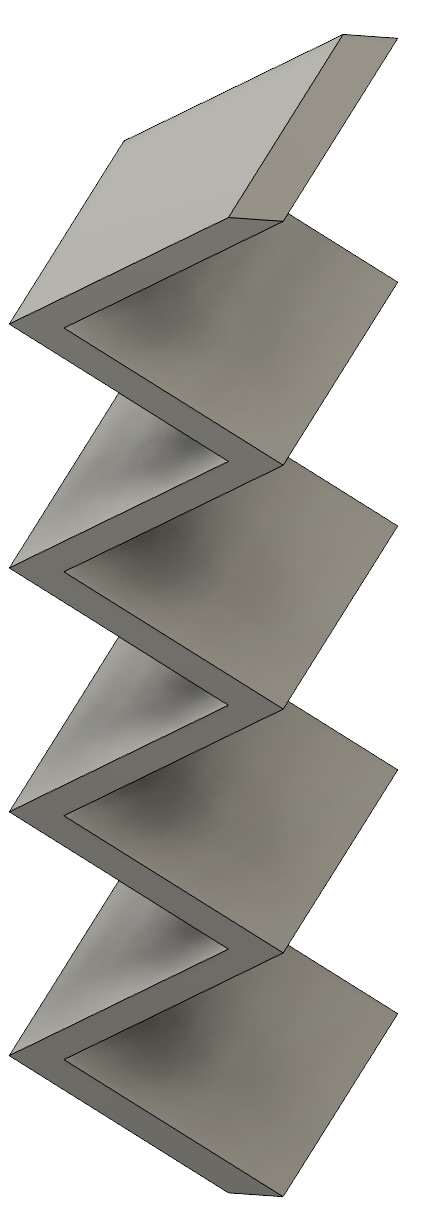
\includegraphics[width=0.2\textwidth]{assets/figures/Protections_laser/Securite_mecanique/Protection_vers_microscope/zigzag_model.jpeg}
    \end{center}
    \captionof{figure}{Modèle 3D avec géométrie en zigzag}
    \label{zigzag_model}
\end{minipage}\hfill
\begin{minipage}[c]{0.48\textwidth}
    \begin{center}
        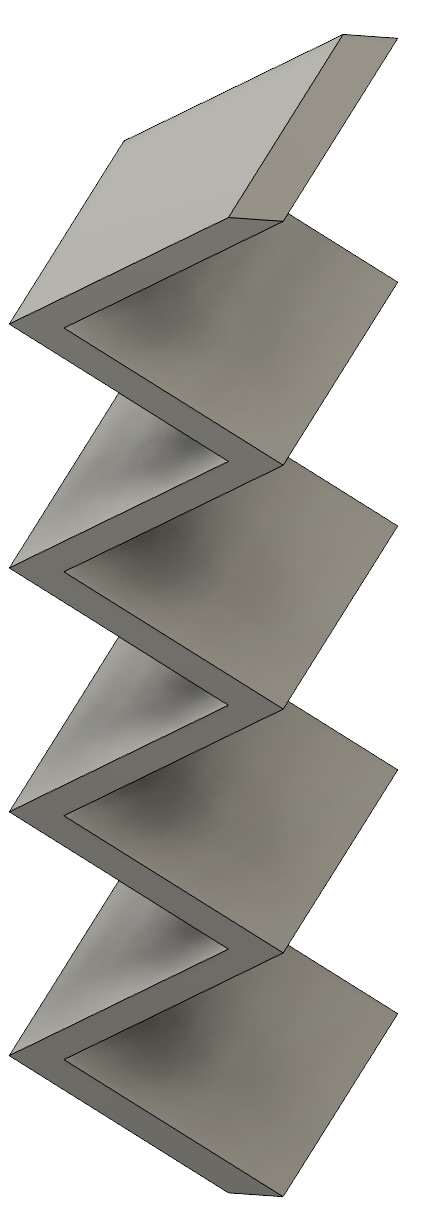
\includegraphics[width=0.2\textwidth]{assets/figures/Protections_laser/Securite_mecanique/Protection_vers_microscope/zigzag_model.jpeg}
    \end{center}
    \captionof{figure}{Impression 3D en TPU du modèle avec géométrie en zigzag}
    \label{zigzag_reel}
\end{minipage}

La solution retenu pour avoir le moins de contraintes possible dans les mouvements a été de faire une conception de protection avec du tissu, associée à des impressions 3D en PLA.

\subsection{Modélisation de la protection}
\begin{minipage}[c]{0.38\textwidth}
    Pour pouvoir mieux comprendre les choix de conception et les étapes faites pour réaliser la protection, la Figure~\ref{model_3D_microscope}, ci-contre, représente la modélisation complète de la protection vers le microscope.
\end{minipage}\hfill
\begin{minipage}[c]{0.58\textwidth}
    \begin{center}
        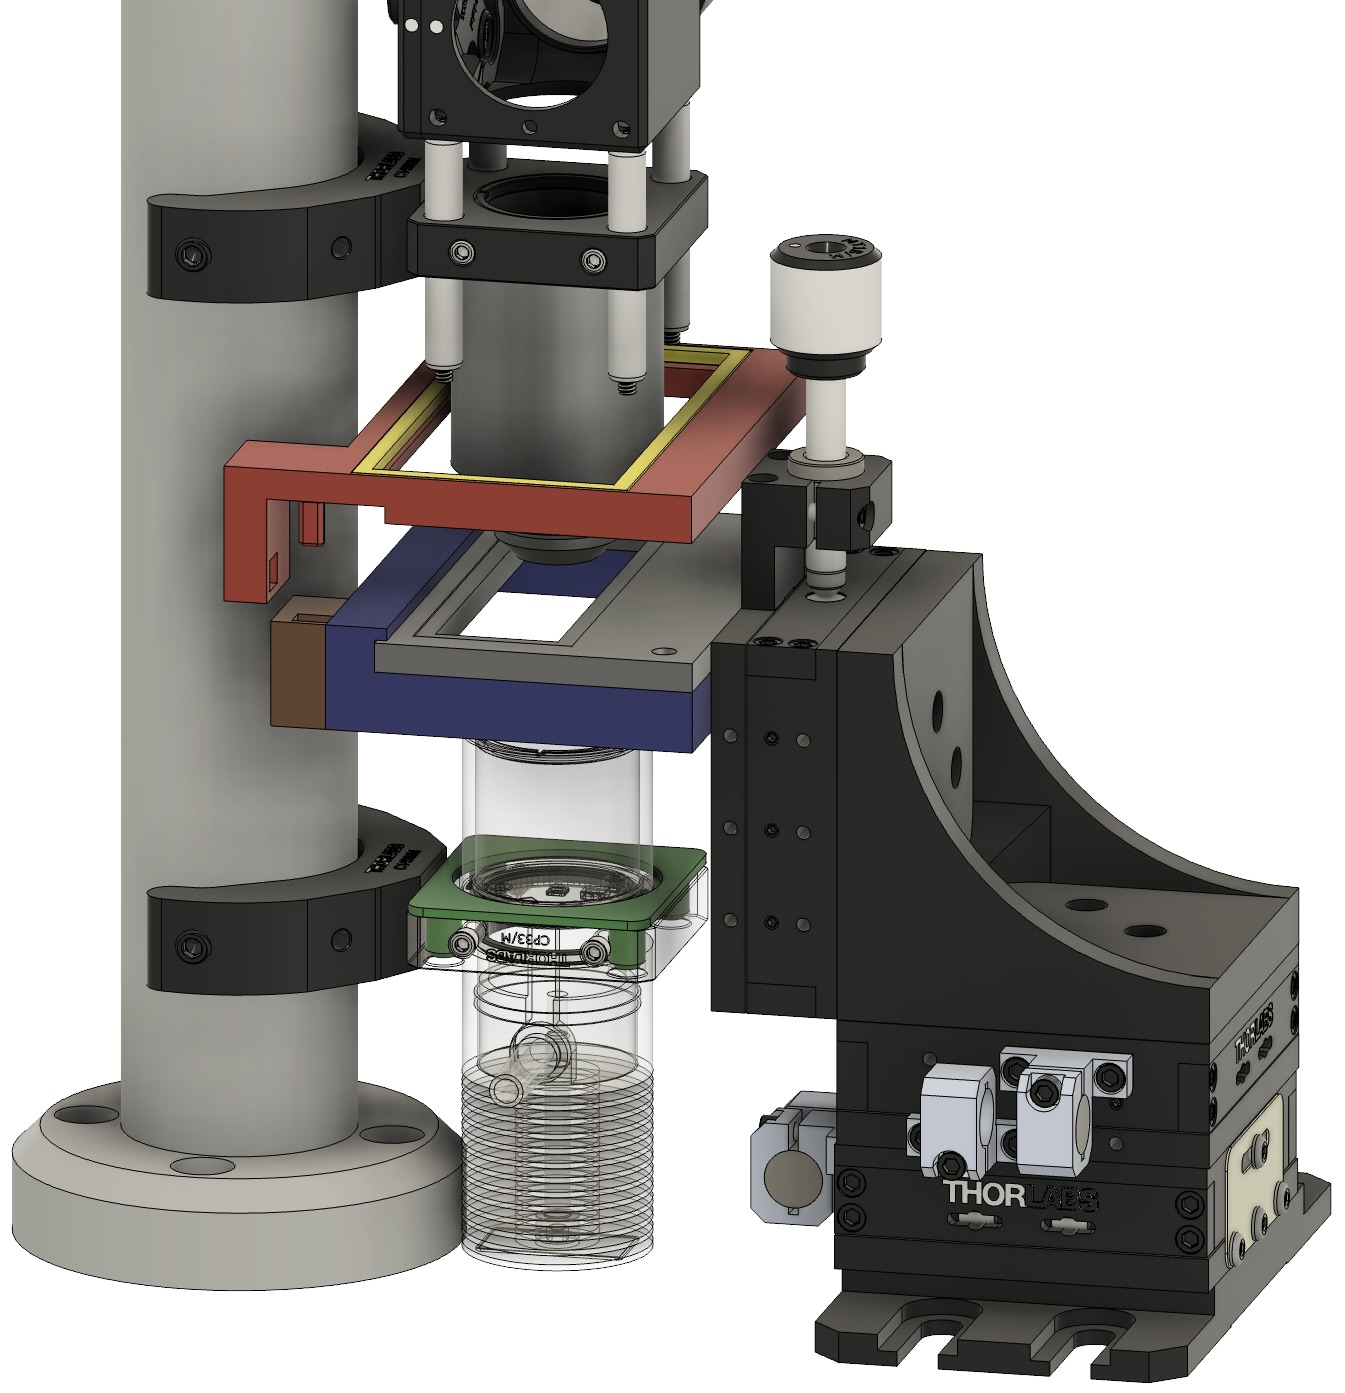
\includegraphics[width=\textwidth]{assets/figures/Protections_laser/Securite_mecanique/Protection_vers_microscope/model_3D.jpeg}
    \end{center}
    \captionof{figure}{Modèle 3D complet de la protection vers le microscope}
    \label{model_3D_microscope}
\end{minipage}

\begin{table}[H]
    \centering
    \caption{Nomenclature des pièces modélisées avec code couleur pour la protection vers le microscope}
    \begin{tabular}{|c|l|}
        \hline
        \textbf{Couleur}                         & \textbf{Nom de la pièce}                             \\
        \hline
        \multicolumn{2}{|c|}{\textbf{Partie inférieure}}                                                \\
        \hline
        \textcolor[RGB]{70, 170, 70}{Vert}       & Support pour fixer le tissu inférieur à la LED       \\
        \textcolor[RGB]{30, 50, 150}{Bleu foncé} & Support pour fixer le tissu inférieur à la platine   \\
        \hline
        \multicolumn{2}{|c|}{\textbf{Partie supérieure}}                                                \\
        \hline
        \textcolor[RGB]{170, 50, 50}{Rouge}      & Support clipsable sur la platine                     \\
        \textcolor[RGB]{120, 70, 30}{Brun}       & Boîtier pour fixer le fin de course                  \\
        \textcolor[RGB]{233, 173, 56}{Jaune}     & Cadre pour fixer le tissu supérieur au support rouge \\
        \hline
    \end{tabular}
    \label{tab:nomenclature_pieces_microscope}
\end{table}

\subsubsection{Partie inférieure}
\begin{minipage}[c]{0.38\textwidth}
    Pour fixer le tissu à LED (pièce \textcolor[RGB]{70, 170, 70}{verte} de la Figure~\ref{model_3D_microscope}), le support montré sur la Figure~\ref{support_inf_tissu_LED}, ci-contre, a été pensé. La plaque, désigné par la flèche \textcolor{red}{rouge}, est une plaque de cage. Ses quatres trous ont été utilisés pour pouvoir fixer le support. les quatres petites vis (flèches \textcolor[RGB]{115, 210, 210}{bleues}), sont des vis sans têtes pour serrer le support en place. Le tissu est pincé entre la plaque et le support imprimé.
\end{minipage}\hfill
\begin{minipage}[c]{0.58\textwidth}
    \begin{center}
        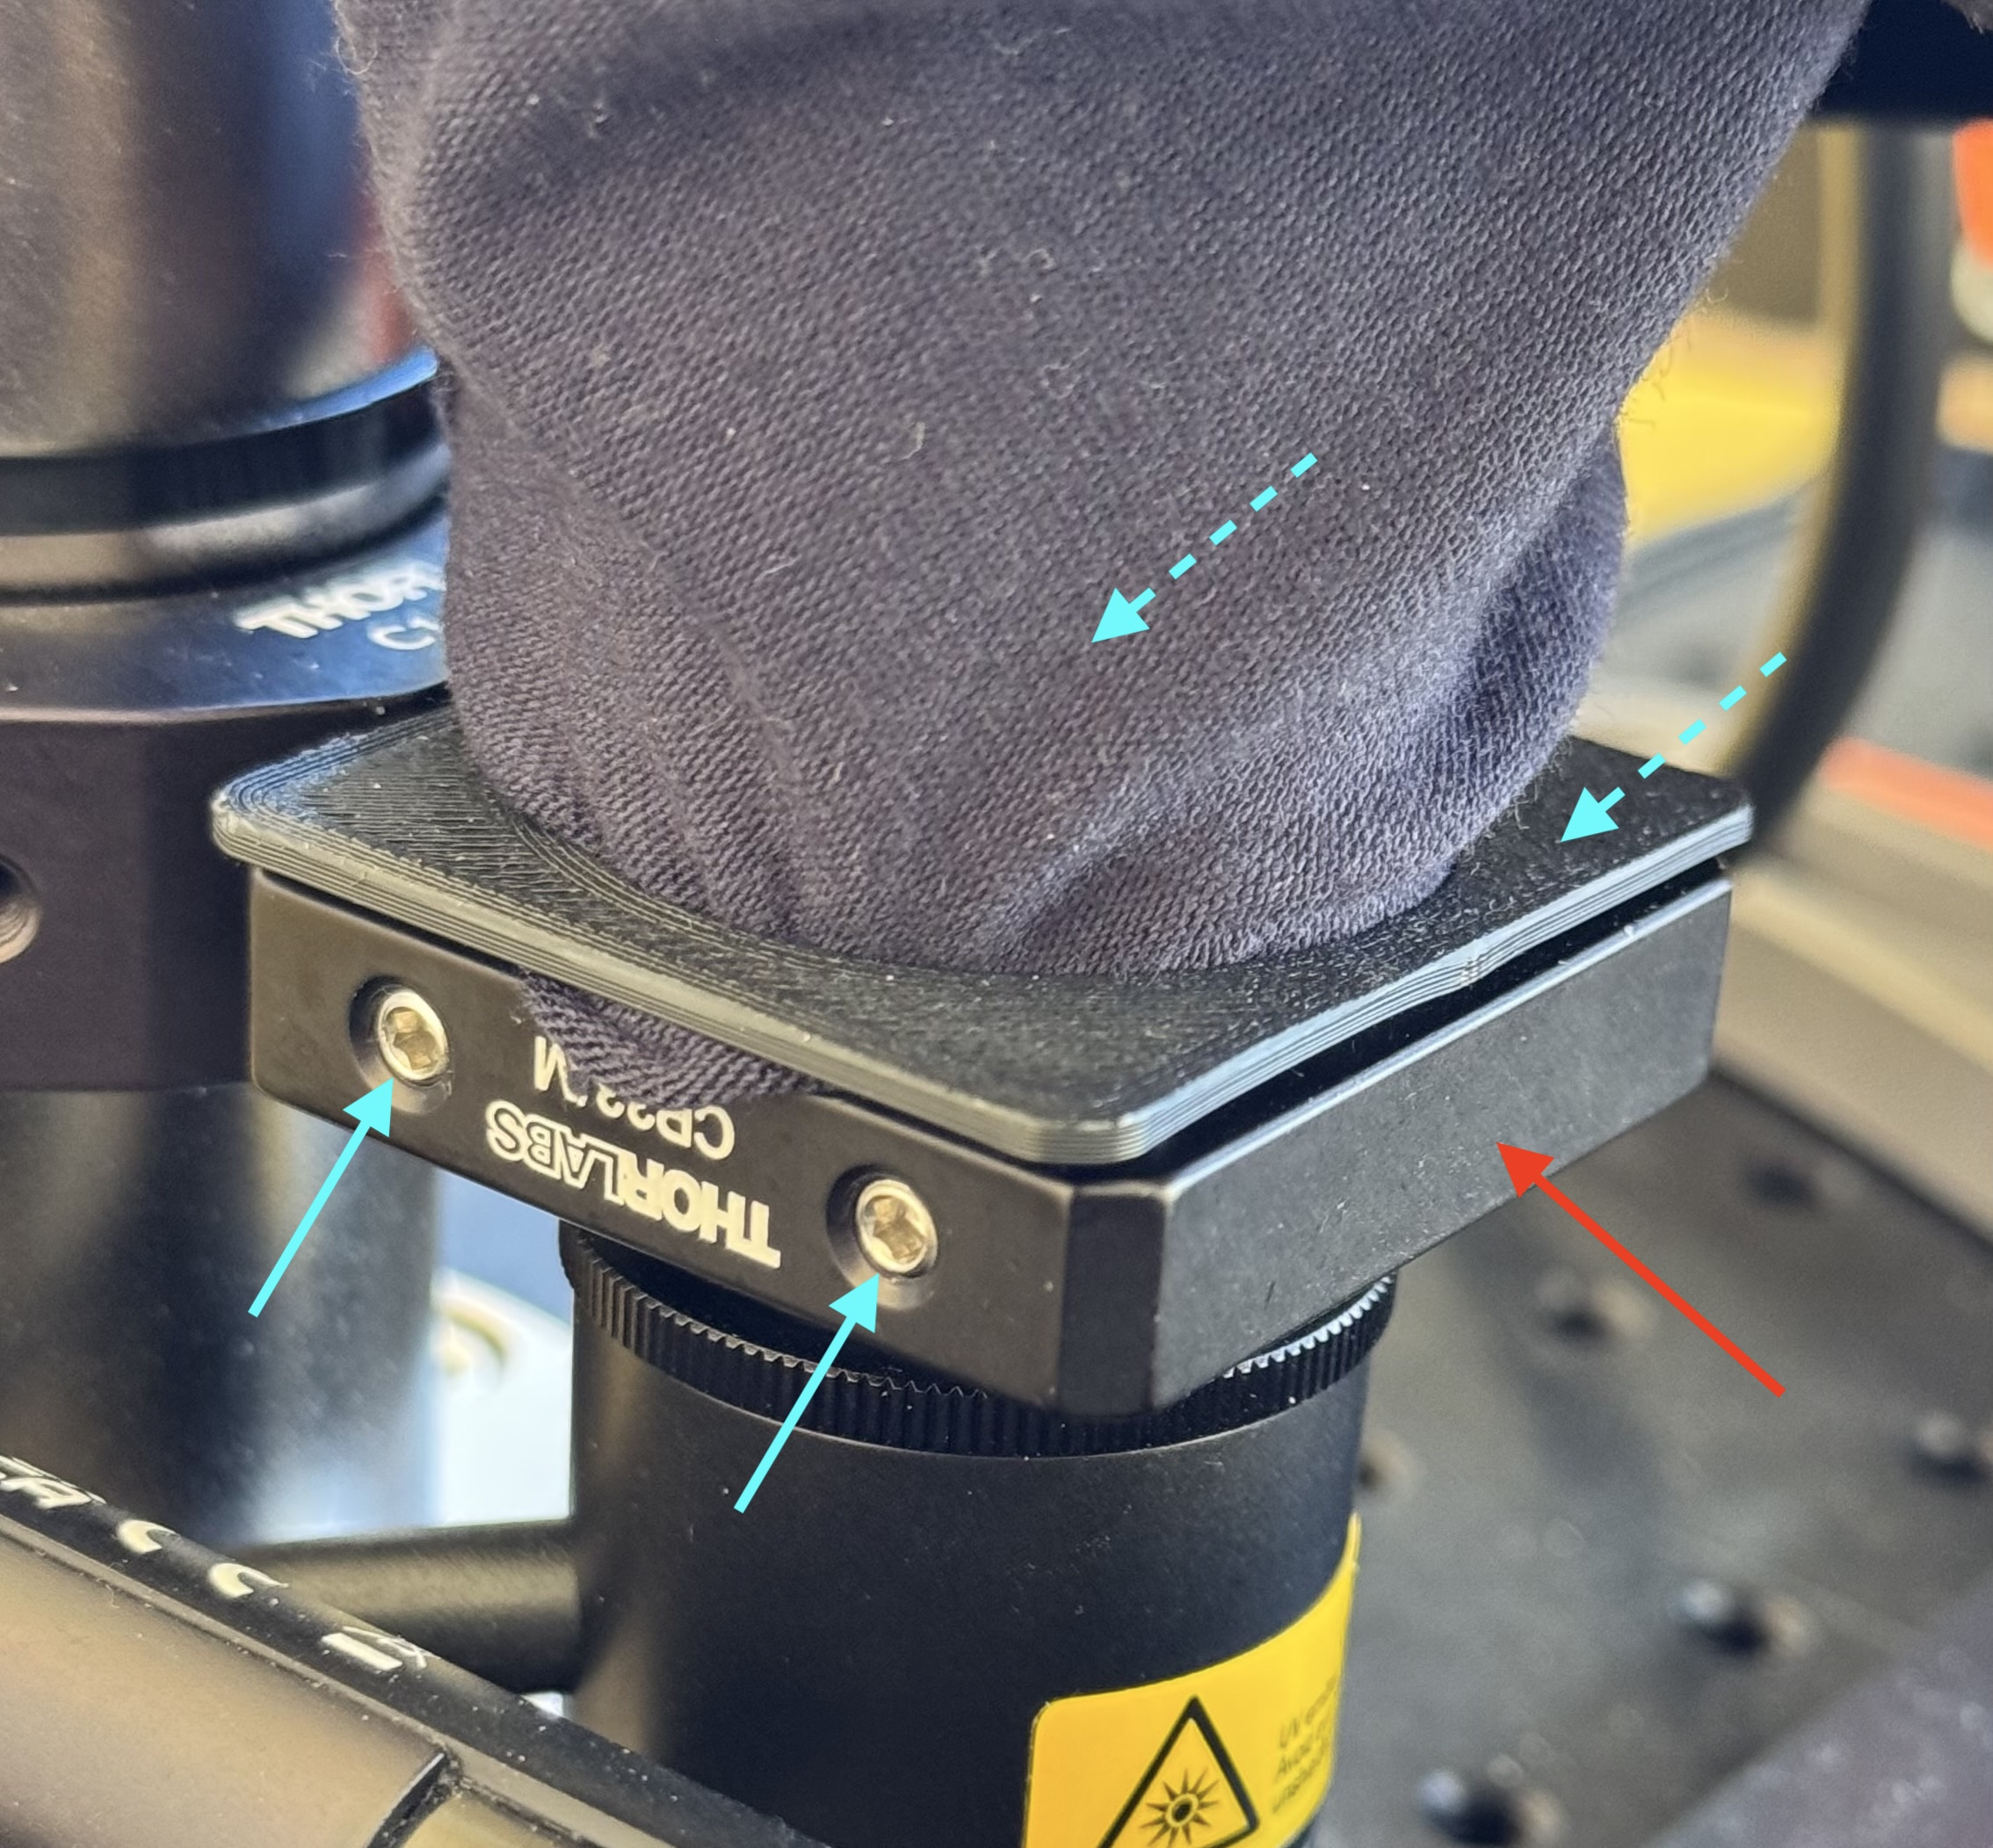
\includegraphics[width=\textwidth]{assets/figures/Protections_laser/Securite_mecanique/Protection_vers_microscope/support_inf_tissu_LED.jpeg}
    \end{center}
    \captionof{figure}{Support pour fixer le tissu inférieur à la lED}
    \label{support_inf_tissu_LED}
\end{minipage}

\begin{minipage}[c]{0.38\textwidth}
    Pour fixer le tissu à la platine (pièce \textcolor[RGB]{30, 50, 150}{bleu foncé} de la Figure~\ref{model_3D_microscope}), le support montré sur la Figure~\ref{support_inf_tissu_platine} (flèche \textcolor{red}{rouge}), ci-contre, a été élaboré. Pour le fixer, les vis montrées par les flèches \textcolor[RGB]{115, 210, 210}{bleues} ont été utilisées. Comme pour la fixation à la LED, ici, le tissu est également coincé entre la platine et le support.
\end{minipage}\hfill
\begin{minipage}[c]{0.58\textwidth}
    \begin{center}
        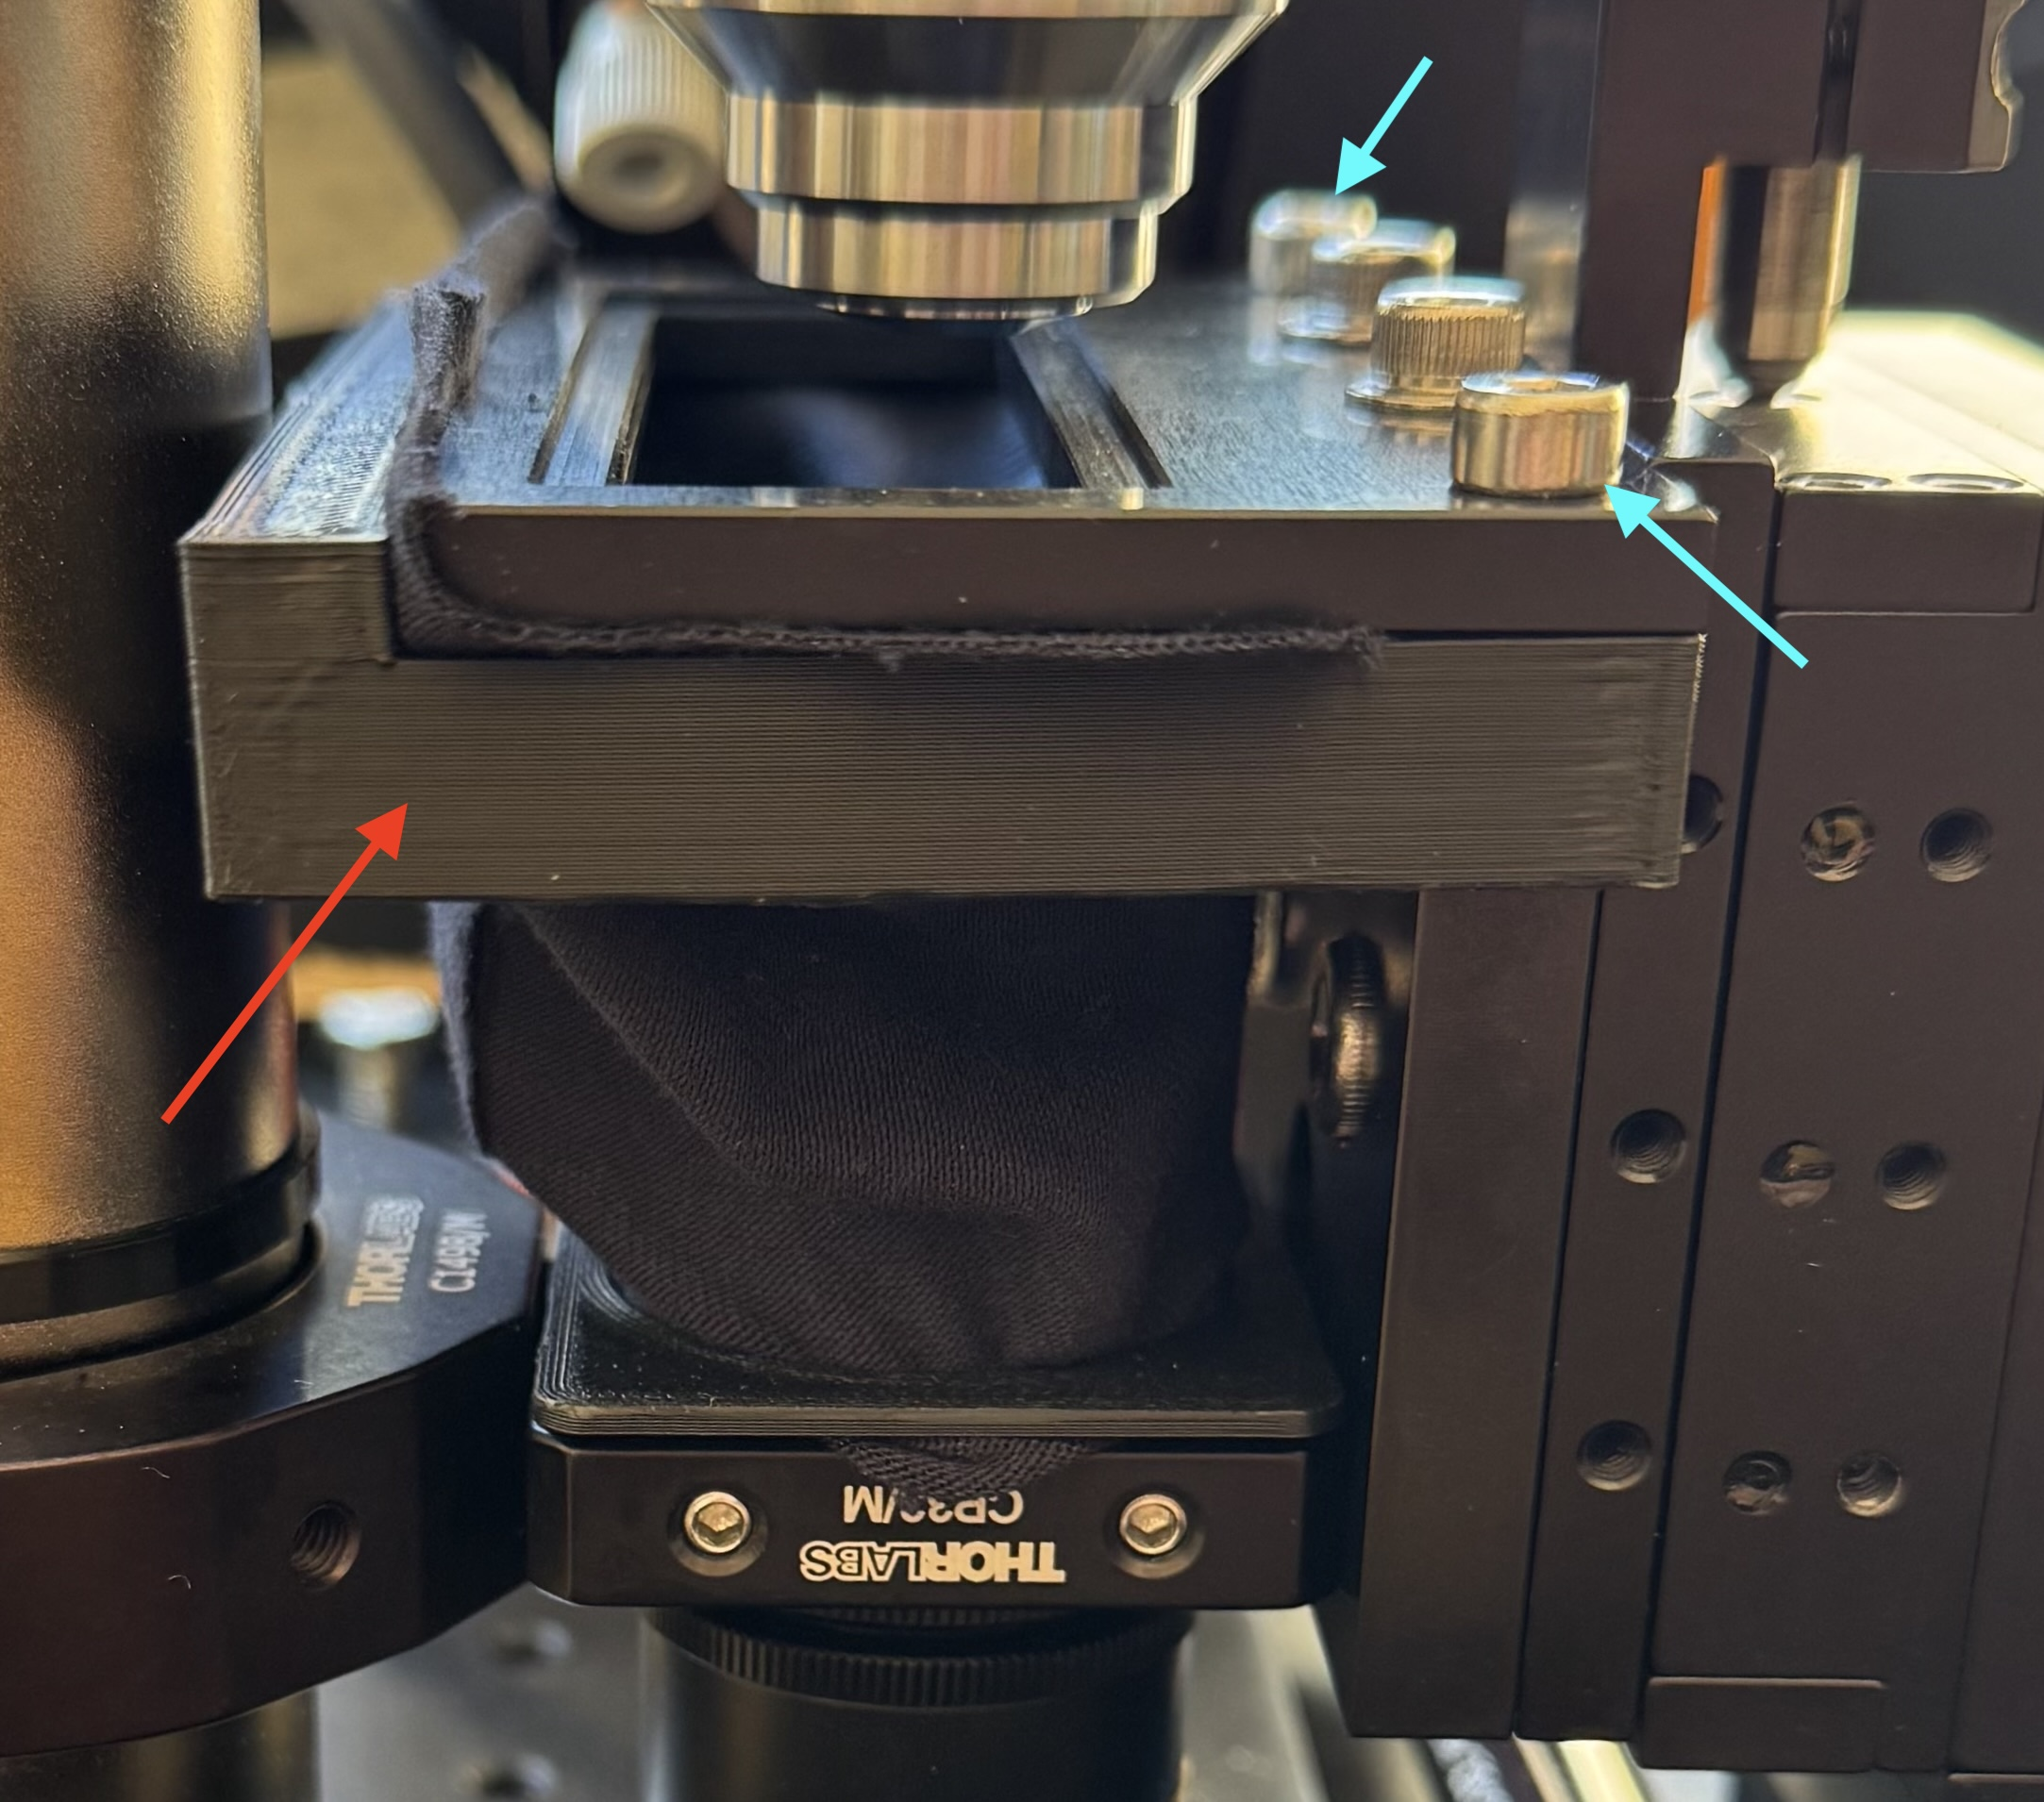
\includegraphics[width=\textwidth]{assets/figures/Protections_laser/Securite_mecanique/Protection_vers_microscope/support_inf_tissu_platine.jpeg}
    \end{center}
    \captionof{figure}{Support pour fixer le tissu inférieur à la platine}
    \label{support_inf_tissu_platine}
\end{minipage}

\subsubsection{Partie supérieure}
